
\documentclass[12pt]{article}

% Layout.
\usepackage[top=1in, bottom=0.75in, left=1in, right=1in, headheight=1in, headsep=6pt]{geometry}

% Fonts.
\usepackage{mathptmx}
\usepackage[scaled=0.86]{helvet}
\renewcommand{\emph}[1]{\textsf{\textbf{#1}}}

% TiKZ.
\usepackage{tikz, pgfplots,tabularx}
\usetikzlibrary{calc}
\pgfplotsset{compat = newest}
 
\pgfplotsset{my style/.append style={axis x line=middle, axis y line=
middle, xlabel={$x$}, ylabel={$y$}, axis equal }}

% Misc packages.
\usepackage{amsmath,amssymb,latexsym}
\usepackage{graphicx}
\usepackage{array}
\usepackage{xcolor}
\usepackage{multicol}
\usepackage{enumerate}

% Commands to set various header/footer components.
\makeatletter
\def\doctitle#1{\gdef\@doctitle{#1}}
\doctitle{Use {\tt\textbackslash doctitle\{MY LABEL\}}.}
\def\docdate#1{\gdef\@docdate{#1}}
\docdate{Use {\tt\textbackslash docdate\{MY DATE\}}.}
\def\doccourse#1{\gdef\@doccourse{#1}}
\let\@doccourse\@empty
\def\docscoring#1{\gdef\@docscoring{#1}}
\let\@docscoring\@empty
\def\docversion#1{\gdef\@docversion{#1}}
\let\@docversion\@empty
\makeatother

% Headers and footers layout.
\makeatletter
\usepackage{fancyhdr}
\pagestyle{fancy}
\fancyhf{} % Clears all headers/footers.
\lhead{\baselineskip 30pt
%\emph{\@doctitle\hfill\@docdate}
\emph{\@docdate\hfill\@doctitle}
\ifnum \value{page} > 1\relax\else\\
\emph{Name: \rule{3.5in}{1pt}\hfill \@docscoring}\fi}
\rfoot{\emph{\@docversion}}
\lfoot{\emph{\@doccourse}}
\cfoot{\emph{\thepage}}
\renewcommand{\headrulewidth}{0pt}%
\makeatother

% Paragraph spacing
\parindent 0pt
\parskip 6pt plus 1pt

% A problem is a section-like command. Use \problem{5} to
% start a problem worth 5 points.
\newcounter{probcount}
\newcounter{subprobcount}
\setcounter{probcount}{0}
\newcommand{\problem}[1]{%
\par
\addvspace{4pt}%
\setcounter{subprobcount}{0}%
\stepcounter{probcount}%
\makebox[0pt][r]{\emph{\arabic{probcount}.}\hskip1ex}\emph{[#1 points]}\hskip1ex}
\newcommand{\thesubproblem}{\emph{\alph{subprobcount}.}}

% Subproblems are an enumerate-like environment with a consistent
% numbering scheme. 
% Use \begin{subproblems}\item...\item...\end{subproblems}
\newenvironment{subproblems}{%
\begin{enumerate}%
\setcounter{enumi}{\value{subprobcount}}%
\renewcommand{\theenumi}{\emph{\alph{enumi}}}}%
{\setcounter{subprobcount}{\value{enumi}}\end{enumerate}}

% Blanks for answers in normal and math mode.
\newcommand{\blank}[1]{\rule{#1}{0.5pt}}
\newcommand{\mblank}[1]{\underline{\hspace{#1}}}
\def\emptybox(#1,#2){\framebox{\parbox[c][#2]{#1}{\rule{0pt}{0pt}}}}

% Misc.
\renewcommand{\d}{\displaystyle}
\newcommand{\ds}{\displaystyle}
\def\bc{\begin{center}}
\def\ec{\end{center}}
\def\be{\begin{enumerate}}
\def\ee{\end{enumerate}}


\doctitle{Math F251X: Quiz 4}
\docdate{September 19, 2024}
\doccourse{UAF Calculus I}
\docversion{v-1 async}
\docscoring{\blank{0.8in} / 25}
\begin{document}
\emph{Please circle your instructor's name:} \hfill Leah Berman  \hfill   Jill Faudree \hfill James Gossell \\

There are 25 points possible on this quiz. Any outside materials (textbook, course notes, calculator) are not allowed.  \emph{For full credit, show all work in a way someone else can follow it.} 
\begin{enumerate}
\item (12 points) Let $f(x)=5x+x^2$.
	\begin{enumerate}
	\item Find $f'(x)$ using the derivative rules from Section 3.3.\\
	\vspace{1in}
	\item Use the definition of the derivative of $f(x)$ (copied below), to confirm that your answer in part (a) is correct.\\
	
	 $\displaystyle f'(x)=\lim_{h \to 0} \frac{f(x+h)-f(x)}{h}.$
	 
	 \vfill 
	 \item Write an equation of the tangent line to $f(x)$ at $x=1.$
	 \vspace{1in}
	 \end{enumerate}
\newpage
\item (6 points) The graph of $G(x)$ is shown below on the left. On the right axes, sketch $G'(x)$, the derivative of $G(x).$  	


\begin{tabularx}{\textwidth}{XXX}
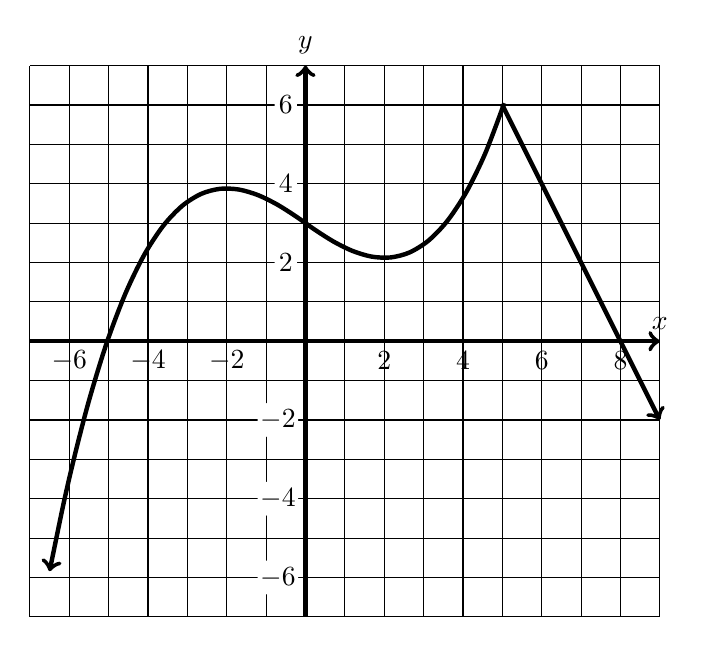
\begin{tikzpicture}[scale = 0.5]
	\draw[ultra thick, ->] (-7, 0) -- (9, 0) node[above] {$x$};
  	\draw[ultra thick, ->] (0, -7) -- (0, 7) node[above] {$y$};
	\foreach \i in {-7,-6,...,7}{
		\draw(-7, \i) -- (9,\i){};}
	\foreach \i in {-7,-6,...,9}{	
		\draw(\i,-7) -- (\i,7){};
		};
	\foreach \i in {-6,-4,-2,2,4,6,8}{
		\node at (\i,-0.5){$\i$};}
	\foreach \i in {-6,-4,-2}{
		\node[fill=white,inner sep=0cm,circle] at (-0.7,\i){$\i$};
		};
	\foreach \i in {2,4,6}{
		\node[fill=white,inner sep=0cm,circle] at (-0.5,\i){$\i$};
		};
	
  	\draw[ultra thick, <-, domain=-6.5:5.05, smooth, variable=\y]  plot ({\y}, {(0.02)*(2*\y^3+3*\y^2-36*\y)+3});
	\draw[ultra thick, ->] (5,6) -- (9,-2);
	\end{tikzpicture}
&
\begin{tikzpicture}[scale = 0.5]
	\draw[ultra thick, ->] (-7, 0) -- (9, 0) node[right] {$x$};
  	\draw[ultra thick, ->] (0, -7) -- (0, 7) node[above] {$y$};
	\foreach \i in {-6,-5,...,8}{	
		\draw(\i,-.5) -- (\i,.5){};
		};
	\foreach \i in {-6,-4,-2,2,4,6,8}{
		\node[fill=white, inner sep=0cm] at (\i,-0.5){$\i$};
		%\node[circle,fill=white, inner sep=0cm] at (-0.5,\i){$\i$};
		};
	\end{tikzpicture}

\end{tabularx}

\item (4 points) Suppose  $V(d)$ gives the number of voles on day $d$ where $V$ is measured in 1000's of voles. Interpret each of the expressions below using complete sentences. Be sure to include units.
	\begin{enumerate}
	\item $V(15) =25.$
\vfill
	\item $V'(15)=0.54.$
\vfill
	\end{enumerate}
\item (3 points) Use the Product Rule to find the derivative of $\; f(x)=\sqrt{x}\sin(x).$ (Write your answer in a reasonably, cleaned-up way.)
\vfill

\end{enumerate}
\end{document}



